date : 23 januari 2024

\subsubsection{Sample and hold}
\begin{figure}[H]
    \centering
    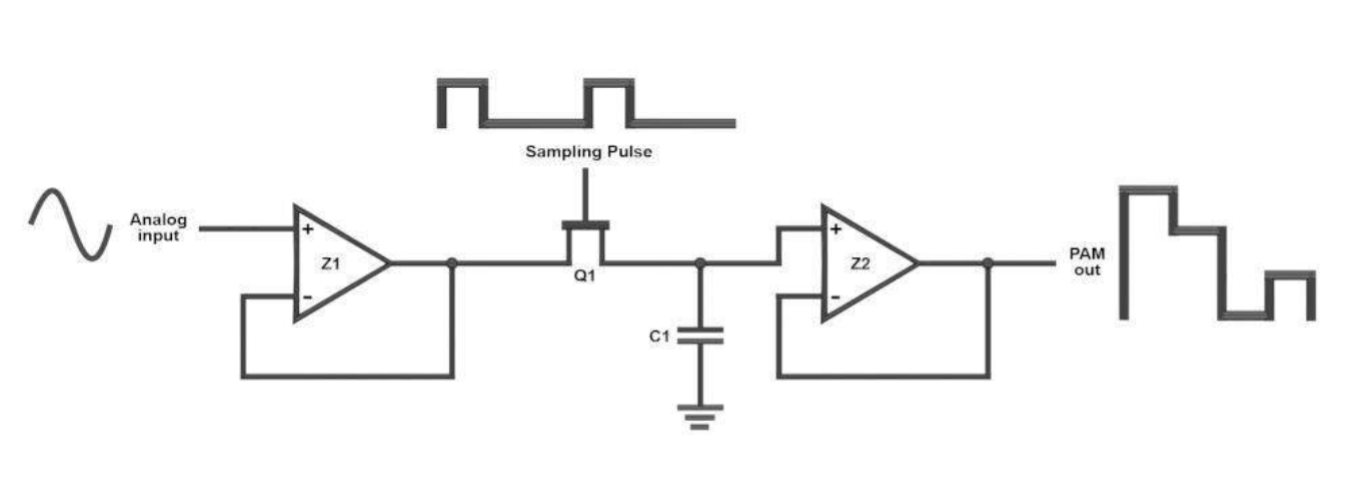
\includegraphics[scale=0.7]{Sample and hold.png}
    \caption*{Sample and hold adc}
    \end{figure}

\subsubsection{Flash ADC}
\begin{figure}[H]
    \centering
    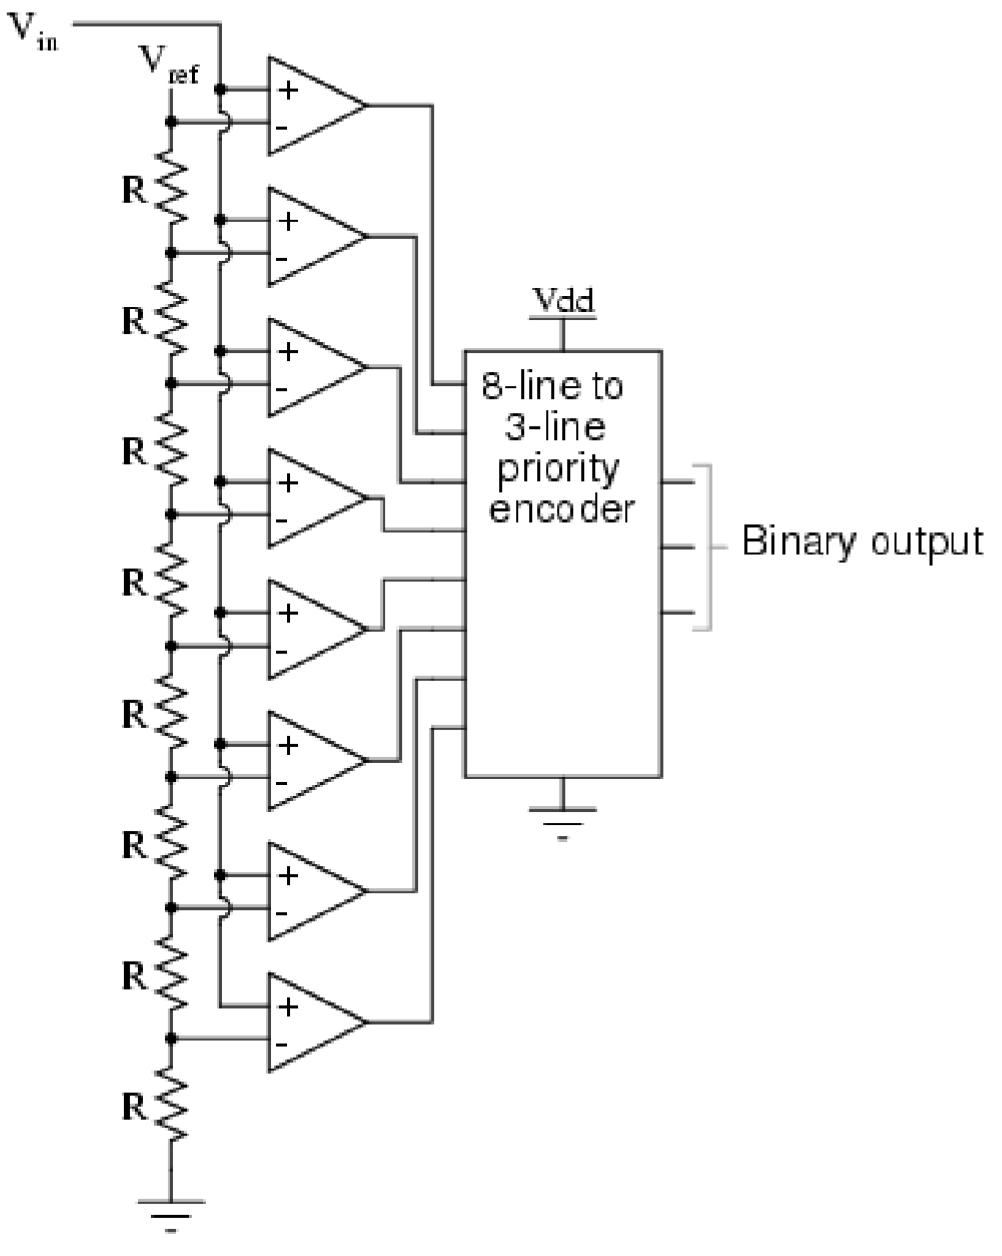
\includegraphics[scale=0.6]{Flash ADC.png}
    \caption*{Flash ADC}
    \end{figure}

Bestaat uit een serie van comparatoren. Iedere comparator vergelijkt het ingangssignaal met een eigen unieke referentiespanning.\\
De uitgangen worden met wat digitale logica (priority encoder)
gebruikt omgezet in een binair signaal.\\
voordelen:
\begin{itemize}
    \item Eenvoudige manier van werken
    \item Snelste manier van omzetten; de beperking zit alleen in propagatie vertraging.
\end{itemize}
nadelen:
\begin{itemize}
    \item LAge resolutie
    \item relatief duur
    \item Voor ieder extra output bit zijn er 2x zo veel comparatoren nodig.
\end{itemize}

\subsubsection{Dual slope ADC}
\begin{figure}[H]
    \centering
    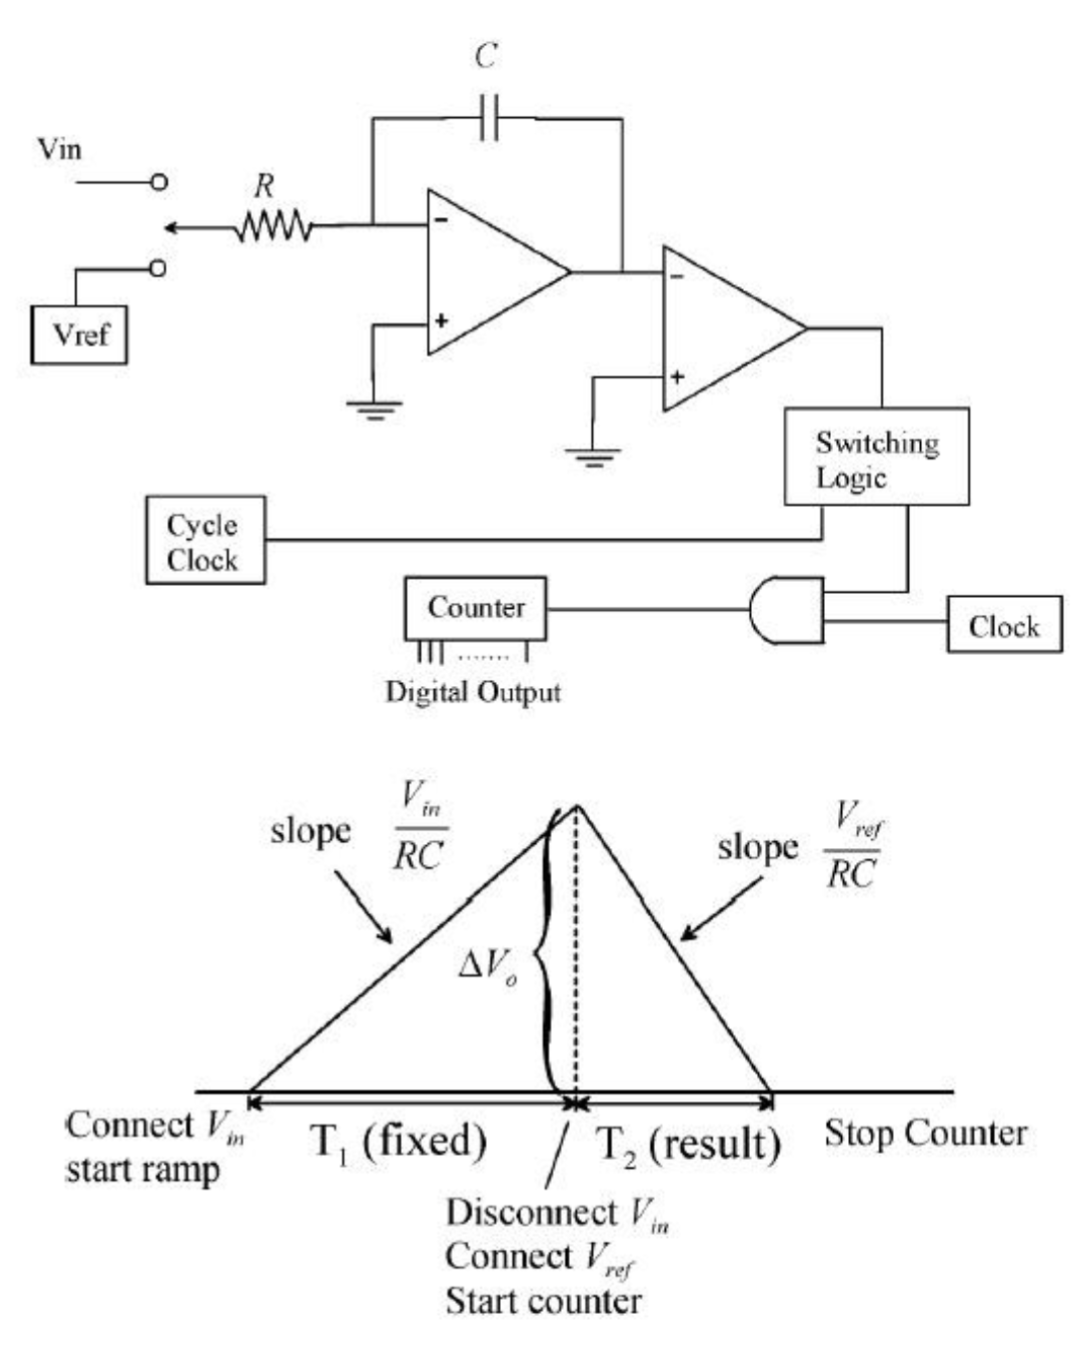
\includegraphics[scale=0.5]{Schermafbeelding 2024-01-23 131007.png}
    \caption*{Dual slope ADC}
    \end{figure}
Het ingangssignaal bepaalt de mate van laden\\
Dan schakelt de ingang naar het referentie voltage en ontlaad; deze tijd wordt gemeten en is een maat voor de spanning\\
Door integratie over tijd hebben we bijna geen last van ruis (alleen van de comparator!!)\\
Na het schakelen met een bekende negatieve ingangsspanning berekenen we de (de)integratie tijd en hebben we een maat voor de ingangsspanning\\
voordelen
\begin{itemize}
    \item Het ingangssignaal wordt gemiddeld
    \item Minder last van ruis dan andere type ADC
    \item Hoge resolutie
\end{itemize}
nadelen:
\begin{itemize}
    \item traag
    \item De kwaliteit van de referentie en de comparator bepaalt de kwaliteit van de schakeling
\end{itemize}

\subsubsection{Succesive Approximation ADC}
\begin{figure}[H]
    \centering
    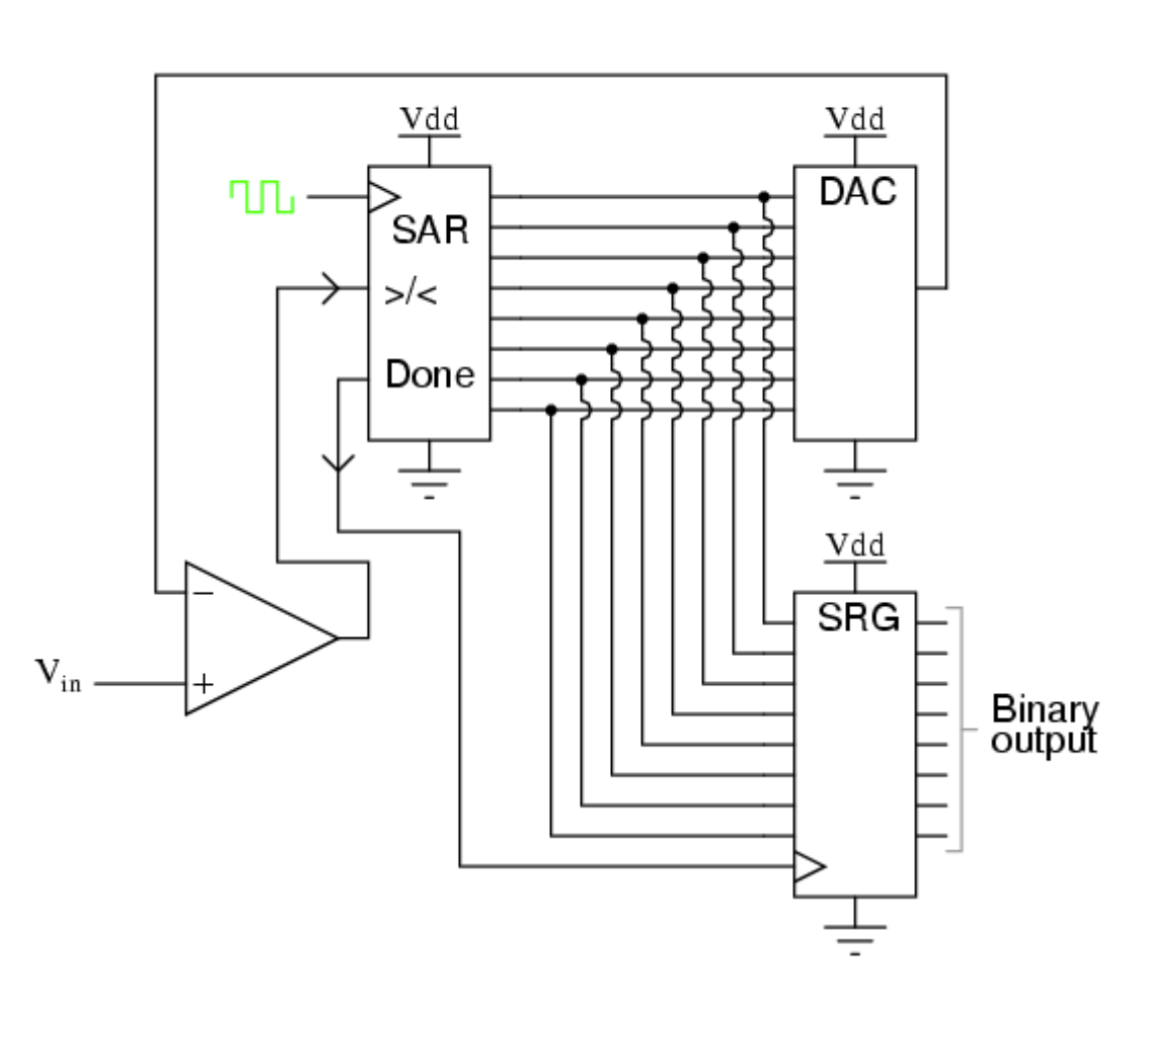
\includegraphics[scale=0.6]{Successive Approximation ADC.png}
    \caption*{Succesive Approximation ADC}
    \end{figure}
A Successive Approximation Register (SAR) is added to the circuit\\
Instead of counting up in binary sequence, this register counts by trying all values of bits starting with the MSB and finishing at the LSB.\\
The register monitors the comparators output to see if the binary count is greater or less than the analog signal input and adjusts the bits accordingly
voordelen:
\begin{itemize}
    \item je kan hem sneller maken door minder bitjes te gebruiken
    \item redelijk hoge snelheden mogelijk
    \item redelijke precisie in vergelijk met andere converters
    \item Betaalbaar en veel kwaliteit
\end{itemize}
nadelen:
\begin{itemize}
    \item kan slecht tegen ruis
    \item Hoe meer bits hoe langzamer de converters
    \item Snelheid beperkt tot ~ 5Msps
\end{itemize}

\subsubsection{Conclusie}
\begin{figure}[H]
    \centering
    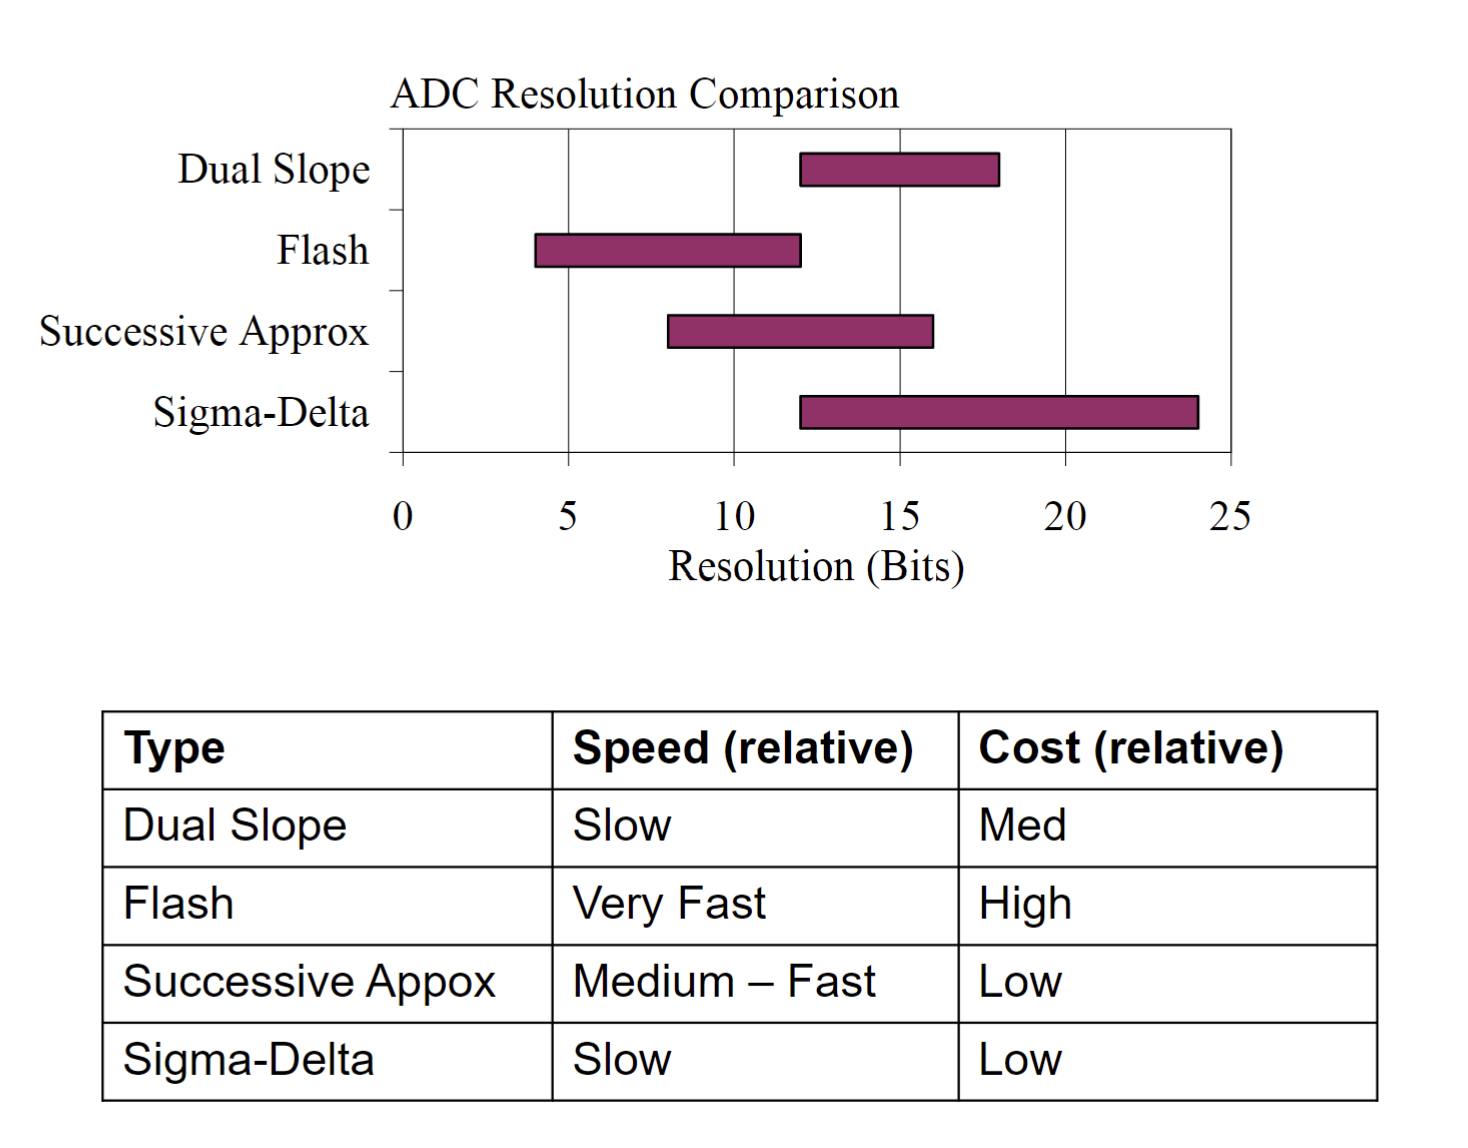
\includegraphics[scale=0.7]{ADC Types Comparison.png}
    \caption*{ADC Types Comparison}
    \end{figure}
    